% PIXIE
% PIXIE.tex

\documentclass[12pt,UTF8]{ctexbook}

% 设置纸张信息。
\usepackage[a4paper,twoside]{geometry}
\geometry{
	left=25mm,
	right=25mm,
	bottom=25.4mm,
	bindingoffset=10mm
}

% 设置字体,并解决显示难检字问题。
\xeCJKsetup{AutoFallBack=true}
\setCJKmainfont{SimSun}[BoldFont=SimHei, ItalicFont=KaiTi, FallBack=SimSun-ExtB]

% 目录 chapter 级别加点(.)。
\usepackage{titletoc}
\titlecontents{chapter}[0pt]{\vspace{3mm}\bf\addvspace{2pt}\filright}{\contentspush{\thecontentslabel\hspace{0.8em}}}{}{\titlerule*[8pt]{.}\contentspage}

% 设置 part 和 chapter 标题格式。
\ctexset{
	chapter/name={第,章},
	chapter/number={\chinese{chapter}}
}

% 图片相关设置。
\usepackage{graphicx}
\graphicspath{{Images/}}

% 设置署名格式。
\newenvironment{shuming}{\hfill\zihao{4}}

% 注脚每页重新编号,避免编号过大。
\usepackage[perpage]{footmisc}

\title{\heiti\zihao{0} PIXIE}
\author{}
\date{}

\begin{document}

\maketitle
\tableofcontents

\frontmatter

\mainmatter

\chapter{Pixie}

Pixie 2 CW Transceiver 由美国 HAM W7AMX 设计,BD6CR 引进国内。

Pixie 意为“小精灵、小仙子”,BD6CR 音译为“皮鞋”。

可能是世界上最简单的电报收发信机,只是 2 个常用三极管与一个常见的 LM386 音频功放 IC 就完成了 80 米业余波段(3.5MHz--3.9MHz)或 40 米业余波段(7.0MHz--7.1MHz)200mW 发信机与直放接收机的组合。(可通过更换晶体振荡器和电感电容改变波段。)输出功率 100--300mW 。

利用这么简陋的机器,不少美国和日本的爱好者成功与几百公里外的业余无线电台进行了双向通信并进行了 QSL 卡片确认。山东威海的 BD4OS 于 10 月 15 日晚 10 点左右使用改进过的“皮鞋”以 600mW 左右的输出功率与几百公里外济南的 BA4IN 完成了 CW/SSB 混合模式双向通信。

\begin{figure}[htbp]
	\centering
	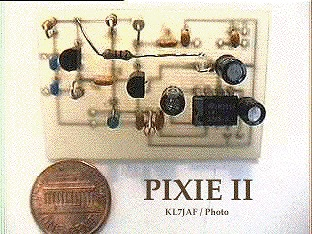
\includegraphics[width=0.7\linewidth]{pixie2}
	\caption{Pixie 机照片与电路图}
	\label{fig:1}
\end{figure}

\textbf{\begin{figure}[htbp]
		\centering
		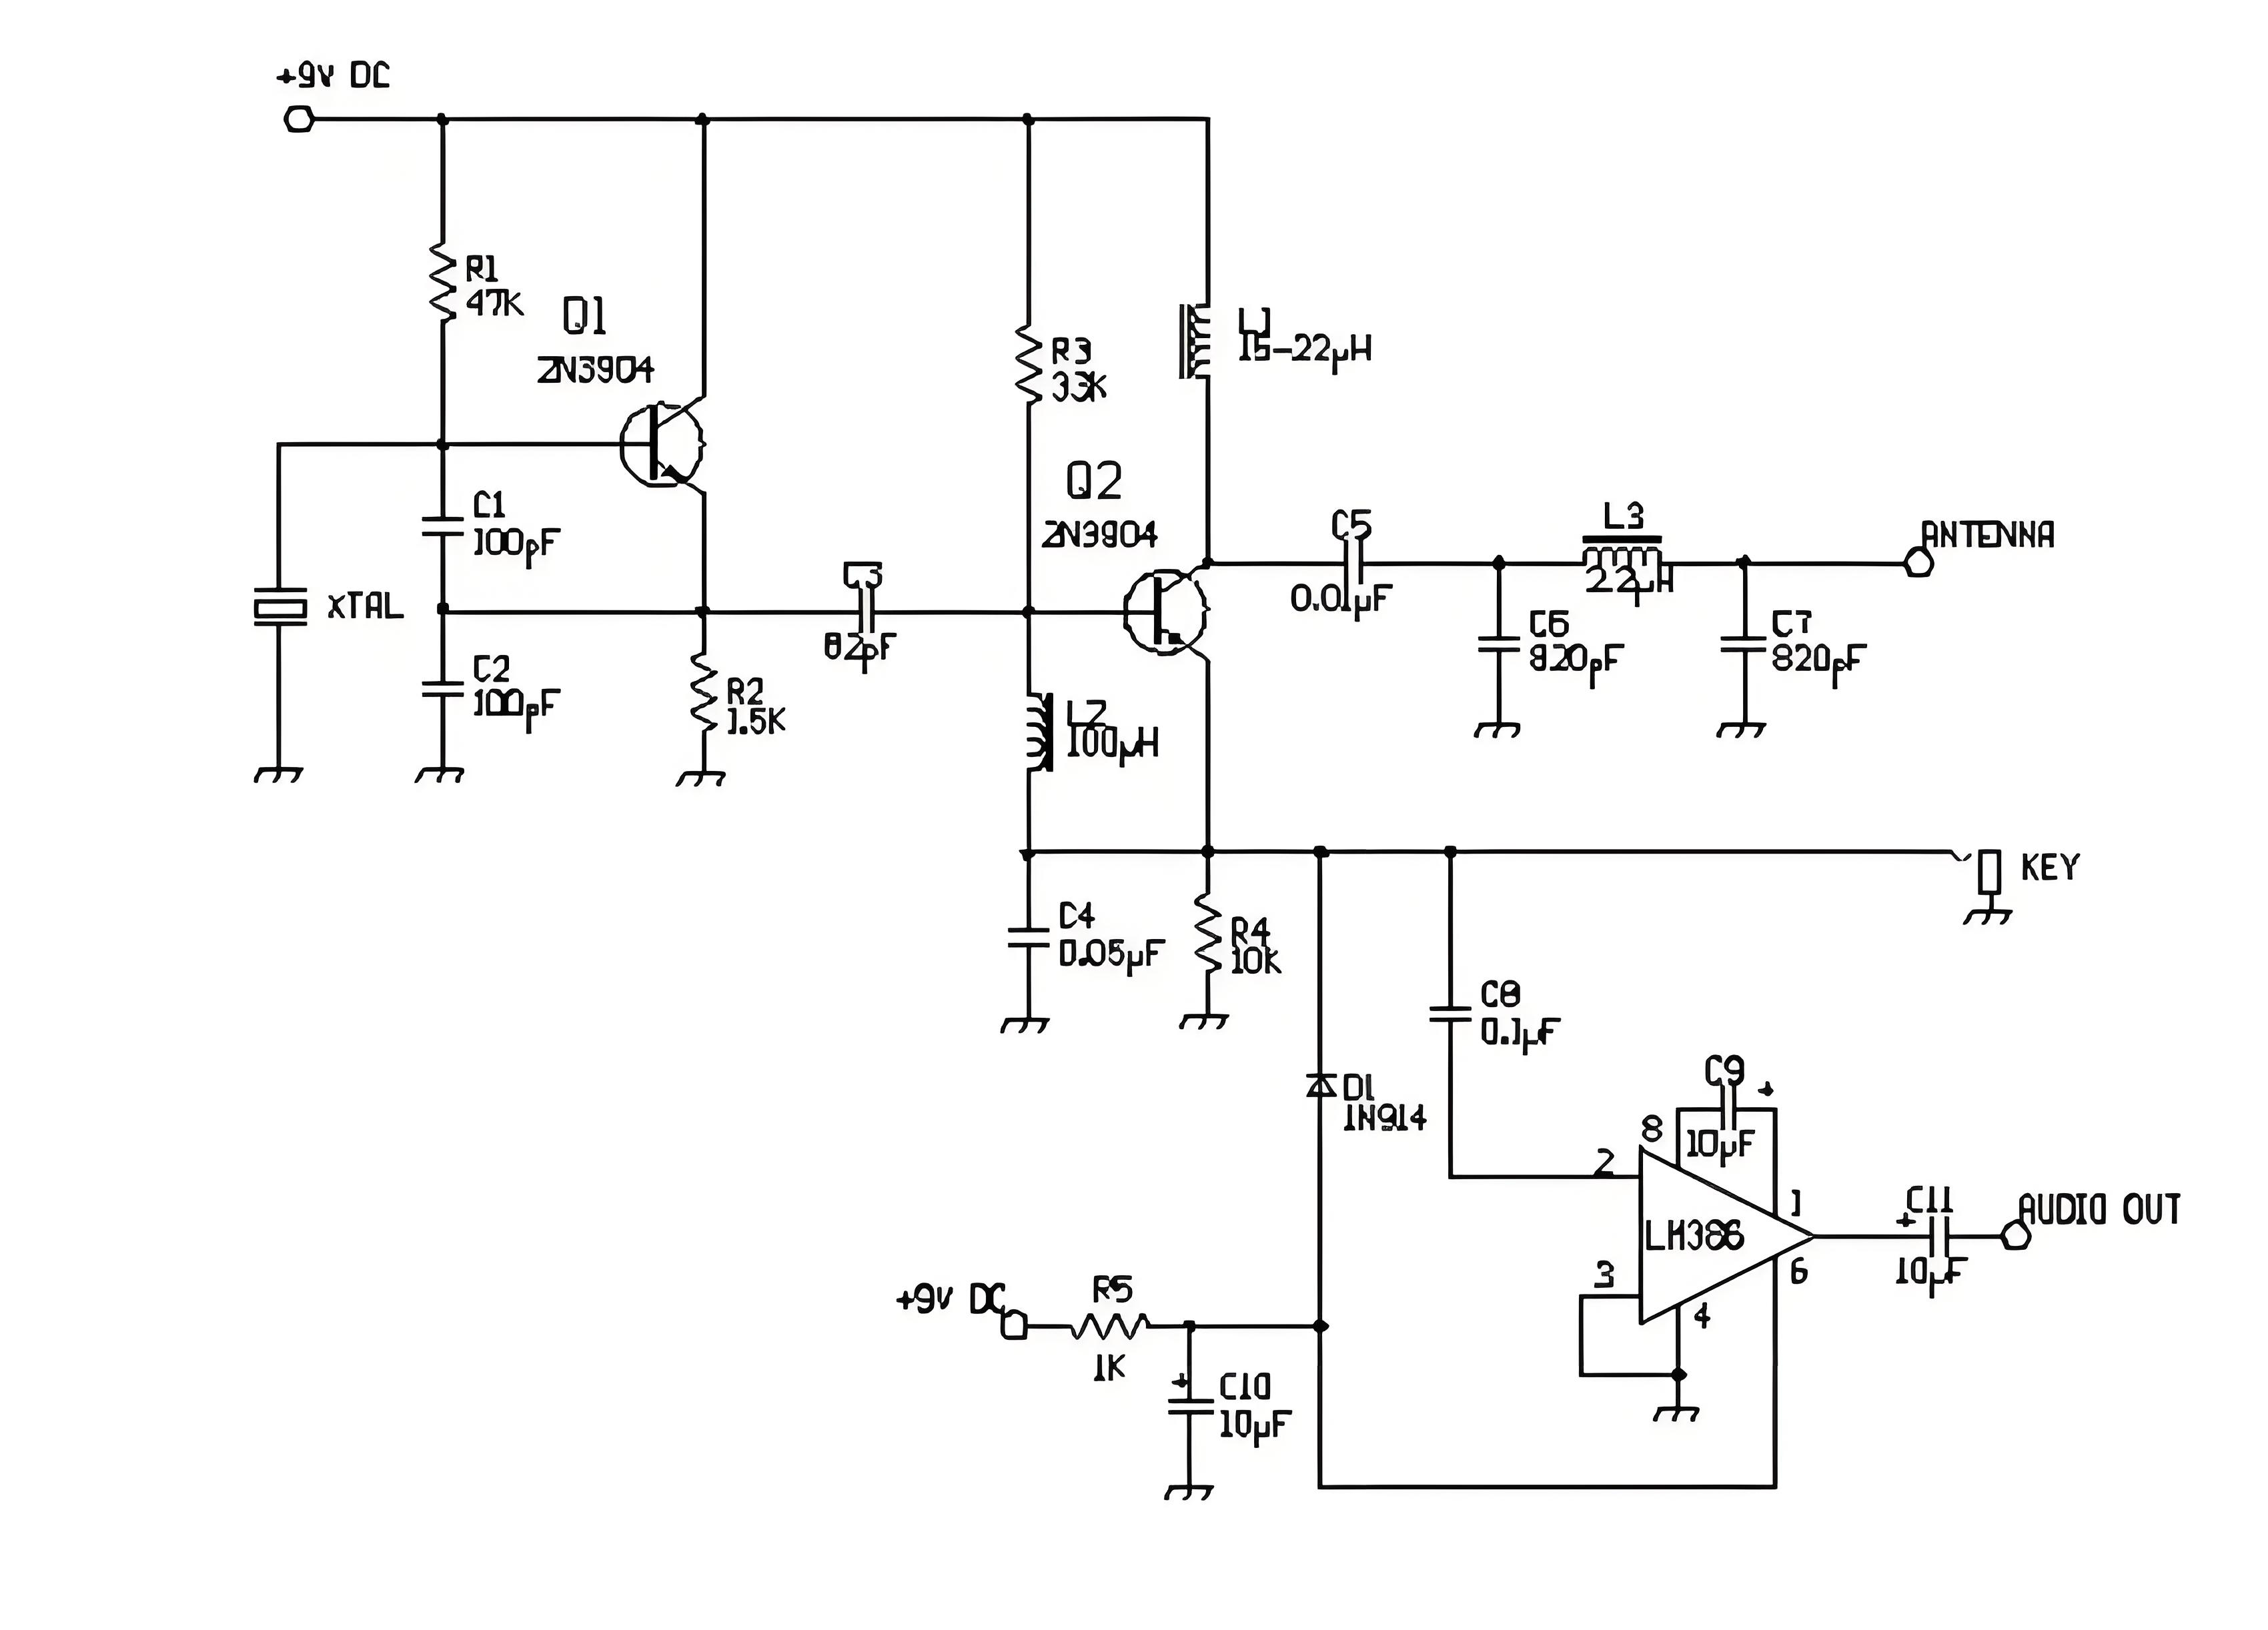
\includegraphics[width=1\linewidth]{Pix2sch}
		\caption{电路图}
		\label{fig:1}
\end{figure}}

\begin{figure}[htbp]
	\centering
	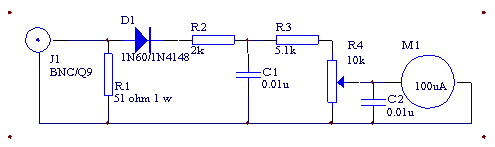
\includegraphics[width=0.7\linewidth]{hfpm}
	\caption{带 1W 假负载的高频功率表}
	\label{fig:1}
\end{figure}


\backmatter



\end{document}